%%%%%%%%%%%%%%%%%%%%%%%%%%%%%%%%%%%%%%%%%
% ATS-Friendly Two-Column CV Template (Custom 70-30 Layout)
%%%%%%%%%%%%%%%%%%%%%%%%%%%%%%%%%%%%%%%%%

\documentclass[9pt, a4paper]{article}
\usepackage[a4paper, margin=0.30in, top=0.2in, bottom=0.2in]{geometry}
\usepackage{fontawesome5}
\usepackage{tabularx}
\usepackage{enumitem}
\usepackage{graphicx}
\usepackage[hidelinks]{hyperref}
\usepackage{amsmath}
\usepackage{xcolor}
\usepackage{tikz}
\usetikzlibrary{shapes.geometric}

\definecolor{sectionblue}{rgb}{0.1, 0.3, 0.6}
\pagestyle{empty}
\setlength{\parindent}{0pt}

\newcommand{\cvsection}[1]{%
	\vspace{2pt}\par
	{\Large\bfseries\color{sectionblue}#1}\par
	\vspace{2pt}\hrule\vspace{6pt}
}

\newcommand{\cvsubsection}[3]{%
	\par {\large\bfseries #1} \hfill {\bfseries #2} \par {\textit{#3}} \vspace{4pt}
}

\newcommand{\jobsection}[3]{%
	\par {\large #1} \hfill {\bfseries #2} \par {\textit{#3}} \vspace{4pt}
}

\newcommand{\cvproject}[1]{%
	\par {{\bfseries{\textit{#1}}}} \par \vspace{4pt}
}

\begin{document}
	
	%---------------- HEADER ----------------
	\begin{center}
		{\Huge\bfseries Bruno Guzzo}\par
		\vspace{4pt}
		{\Large Cloud Engineer | AI \& ML Specialist}
	\end{center}
%	\vspace{5pt}
	
	%---------------- TWO-COLUMN LAYOUT USING MINIPAGE (70-30) ----------------
	\begin{minipage}[t]{0.65\linewidth}
		\vspace{0pt} % Top-align
		
		%---------------- LEFT COLUMN ----------------
		\cvsection{Work Experience}
		
		\jobsection{\textbf{AI Specialist} (Mid-Senior Consultant)}{January 2025 -- Present}{\href{https://www.reply.com/go-reply/en}{Go Reply, Turin}}
		
		\begin{itemize}[leftmargin=*, nosep]
			% MISE - BIANCA
			\item \footnotesize Coordinated a multi-company effort to gather customer requirements for a \textbf{research-oriented healthcare platform}, enabling centralized and rapid clinical or genomic \textbf{data retrieval}. Lead project key phases form defining a complete \textbf{functional analysis} document, design a \textbf{cloud-native architecture} and implementation throught sprint planning.      
			
			% Azimut
			\vspace{5pt}
			\item \footnotesize Directed a cross-functional team of developers in delivering a \textbf{B2C cloud-native mobile application} enabling after-sales support, digital documentation access via \textbf{Gen-AI RAG chat-bot} and seamless multi-cloud \textbf{CRM integration}. Guided the adoption of a distributed serverless \textbf{micro-services} architecture coordinated using \textbf{Google Pub/Sub} to enforce \textbf{fault isolation} and scalability. 
			
			% FAO 
			\vspace{5pt}
			\item \footnotesize Designed and implemented a scalable \textbf{legal treaties search engine} and \textbf{RAG solution} using \textbf{Vertex AI} and \textbf{BigQuery} with a highly efficient and concurrent data ingestion pipeline, enabling insight generation and optimization of customer workflow. 
			Successfully improved data processing speed by \textbf{94\%} after adopting a serverless cloud-native master/worker architecture relying on \textbf{Cloud Task} and \textbf{Cloud Run} for concurrent workloads distribution.      
			
			% Advisory & business development	
			\vspace{5pt}		
			\item \footnotesize Advised clients on \textbf{AI and agent-based system} integration, facilitating the adoption of Google Cloud enterprise ecosystem via \textbf{custom-tailored RFP solutions} to improve critical business processes.
			Increased client adoption rate of Vertex AI by \textbf{30\%}.  
			
			% FAO Mgmt
			\vspace{5pt}
			\item \footnotesize Managed \textbf{strategic client engagement} within the global development industry, coordinating \textbf{multi-project cloud advisory} and \textbf{resource allocation} that mobilized \textbf{20\%} of the BU workforce and drove \textbf{30\%} of unit profitability.
			
			% Development
			\vspace{5pt}
			\item \footnotesize Mentored junior engineers, \textbf{promoted agile best practices} through knowledge-sharing events, and \textbf{coordinated sprint reviews} and retrospectives to accelerate team performance and continuous improvement. 
			Successfully decreased code-review time by \textbf{60\%}.  
		\end{itemize}
		
		\vspace{6pt}
		\jobsection{\textbf{Cloud Engineer} (Consultant)}{June 2022 -- December 2024}{\href{https://www.reply.com/go-reply/en}{Go Reply, Turin}}
		\begin{itemize}[leftmargin=*, nosep]
			
			% Infarm
			\item \footnotesize Contributed to the development of a digital platform for the \textbf{agriculture and food sector}, enhancing \textbf{data collection and analytics} capabilities to support evidence-based decision-making on sustainable farming and antimicrobial resistance. 
			Lead the platform \textbf{migration to Google Cloud} relying on IAC best-practices as full \textbf{Terraform foundation} and \textbf{GCP Fabric} modules to ensure custom service configuration and resources tracking.
			Successfully reduced infrastructural fixed-costs by \textbf{30\%}.
			
			% Dev/Ops
			\vspace{5pt}
			\item \footnotesize Designed efficient multi-stage \textbf{Git-Hub} and \textbf{Git-Lab CI/CD pipeline} for quickest application deployment to production using \textbf{Cloud Build} for \textbf{Docker} image building and a fine-grained configured \textbf{Cloud Run} instance (or Firebase hosting) for computing. Bug-free releases are accomplished leveraging a comprehensive test-cases suite targeting both back-end, using \textbf{Junit} or \textbf{PyTest}, and front-end, using \textbf{Selenium} to mimic end-user actions.       
			
			% Futuri
			\vspace{5pt}
			\item \footnotesize Participated in the implementation and deployment of a \textbf{digital learning solution} in the \textbf{education industry}, delivering scalable and cloud-based features aligned with client innovation goals. Data security and \textbf{GDPR compliance} are guaranteed by the adoption of rigid \textbf{IAM policy} and region locks through the definition of project \textbf{IAC}, using \textbf{Terraform}. 
			
			% Vodafone
			\vspace{5pt}
			\item \footnotesize Modernized a large-scale \textbf{telecommunications cybersecurity platform}, improving scalability and enhancing user experience through \textbf{software architectural refactoring}, cloud integration, and automation to strengthen \textbf{service reliability}. 
		\end{itemize}
		
		\vspace{10pt}\par
		\cvsection{Personal \& Academic Projects}
		
		\cvproject{\href{https://github.com/bGuzzo/msc-ai-ml-thesis-anomaly-detection}{MSc Thesis: Anomaly Detection with Deep Autoencoders}}
		\begin{itemize}[leftmargin=*, nosep]
			\item \footnotesize Developed a novel Autoencoder (AE-SAD) for semi-supervised anomaly detection, significantly improving accuracy (AUC) and reducing training time by addressing class imbalance.
		\end{itemize}
		
		\vspace{5pt}
		\cvproject{\href{https://github.com/bGuzzo/transformer-gnn-link-prediction}{Transformer-GNN for Link Prediction}}
		\begin{itemize}[leftmargin=*, nosep]
			\item \footnotesize Engineered a scalable data pipeline for large-scale graph dataset generation from Wikipedia. Trained and assessed Graph Attention Network (GAT) models for link prediction.
		\end{itemize}
		
		\vspace{5pt}
		\cvproject{\href{https://github.com/bGuzzo/Italian-LLaMA-Project}{LLaMA 3 Fine-Tuning and Evaluation}}
		\begin{itemize}[leftmargin=*, nosep]
			\item \footnotesize Fine-tuned LLaMA 3 on Italian Wikipedia, improving language modeling and developing a RAG-based chatbot for Italian literature.
		\end{itemize}
		
		\vspace{10pt}\par
		\cvsection{Education}
		
		\cvsubsection{MSc, AI \& ML Engineering}{Oct 2022 -- July 2025}{UNICAL, Rende (CS), Italy}
		\cvsubsection{BSc, Computer Engineering}{Oct 2018 -- June 2022}{UNICAL, Rende (CS), Italy}
		
	\end{minipage}%
	\hfill%
	\begin{minipage}[t]{0.32\linewidth}
		\vspace{0pt} % Top-align
		
		%---------------- RIGHT COLUMN ----------------
		\begin{center}
			\begin{tikzpicture}
				\clip (0,0) circle (2.25cm);
				\node at (0,0) {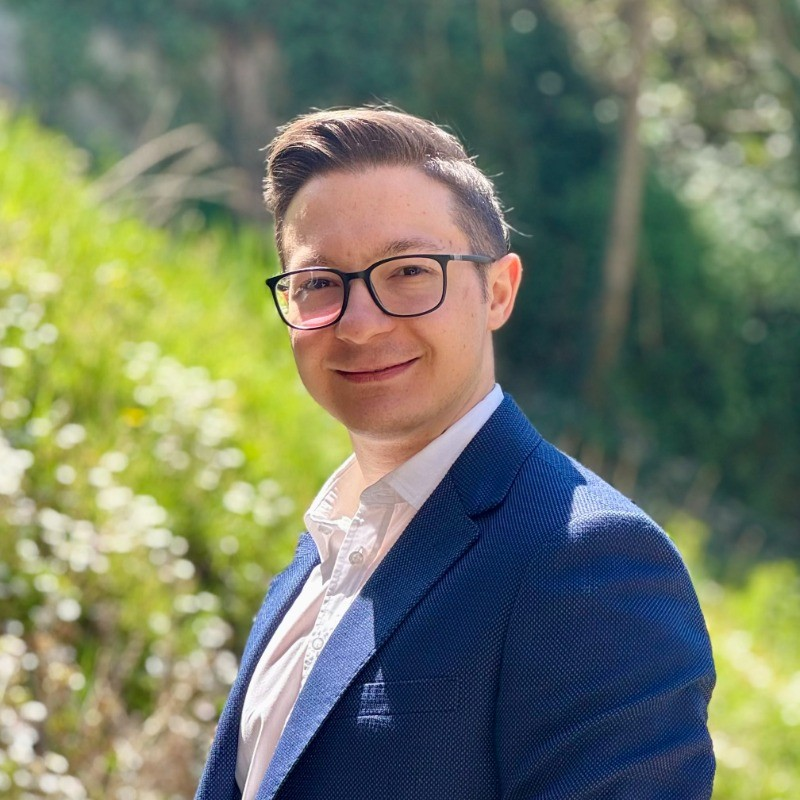
\includegraphics[width=4.5cm]{PICS/me_linkedin.jpeg}};
			\end{tikzpicture}
		\end{center}
%		\vspace{4pt}
		
		\begin{tabularx}{\linewidth}{@{}lX@{}}
			\faBirthdayCake & 13 Jan 2000 \\
			\faPhone & +393398305458 \\
			\faEnvelope & \href{mailto:brunoguzzo18@gmail.com}{brunoguzzo18@gmail.com} \\
			\faGithub & \href{https://github.com/bGuzzo}{github.com/bGuzzo} \\
			\faLinkedin & \href{https://www.linkedin.com/in/guzzobruno/}{linkedin.com/in/guzzobruno} \\
		\end{tabularx}
		\vspace{4pt}
		
		\cvsection{Soft Skills}
		\begin{itemize}[leftmargin=*, nosep, itemsep=2pt]
			\footnotesize
			\item Leadership \& Mentoring
			\item Team \& Project Management
			\item Consulting \& Client Engagement
			\item Agile Methodologies (Scrum)
		\end{itemize}
		\vspace{5pt}
		
		\cvsection{Technical Skills}
		
		{\bfseries Google Cloud} (\textit{Advanced})
		\begin{itemize}[leftmargin=*, nosep, itemsep=2pt]
			\footnotesize
			\item \textbf{Compute}: Cloud Run, App Engine, Cloud Functions, Compute Engine
			\item \textbf{AI/ML}: Gemini, Vertex AI, Agent Builder, ADK, BigQuery ML
			\item \textbf{Data}: BigQuery, Cloud SQL, Firestore, and Firebase Realtime Database, Cloud Storage
			\item \textbf{Infra}: VPC, Load Balancer, IAM, Cloud Armor, Cloud DNS, Cloud CDN, Cloud Task, Cloud Pub/Sub
		\end{itemize}
		\vspace{5pt}
		
		{\bfseries AI \& Machine Learning} (\textit{Academic})
		\begin{itemize}[leftmargin=*, nosep, itemsep=2pt]
			\footnotesize
			\item \textbf{Frameworks}: PyTorch, Langchain, Hugging Face Transformers, PEFT, Unsloth
			\item \textbf{Libraries}: Pandas, NumPy, Scikit-learn, SciPy, NLTK, Sentence-Transformers, FAISS, BitsAndBytes
			\item \textbf{Concepts}: LLM, RAG, NLP, Fine-Tuning (QLoRA), Vector Databases, Embeddings, Anomaly Detection, Time-Series Analysis, Reinforcement Learning, GNNs, CNNs, Autoencoder, Transformer, GPT
		\end{itemize}
		\vspace{5pt}
		
		{\bfseries DevOps} (\textit{Advanced})
		\begin{itemize}[leftmargin=*, nosep, itemsep=2pt]
			\footnotesize
			\item \textbf{IaC}: Terraform, Fabric
			\item \textbf{CI/CD}: Cloud Build, GitLab CI, GitHub Actions, Artifact Registry
			\item \textbf{Containers}: Docker
			\item \textbf{Others}: Linux, Git, Bash scripting
		\end{itemize}
		\vspace{5pt}
		
		{\bfseries Software Development} (\textit{Advanced})
		\begin{itemize}[leftmargin=*, nosep, itemsep=2pt]
			\footnotesize
			\item \textbf{Languages}: Python, Java, C, JavaScript, Typescript, Dart, SQL
			\item \textbf{Frameworks}: Spring Boot, Hibernate, JPA, Flask, Django, SQLAlchemy Angular, React, Flutter
			\item \textbf{Testing}: Selenium, Junit, PyTest
			\item \textbf{Databases}: PostgreSQL, MySQL, NoSQL
			\item \textbf{Others}: Jira, Sprint Planning, Cloud-Native, Design Patterns
		\end{itemize}
		\vspace{7pt}
		
		\cvsection{Languages}
		\begin{itemize}[leftmargin=*, nosep, itemsep=2pt]
			\item \textbf{Italian}: Native
			\item \textbf{English}: B2, Cambridge certified
		\end{itemize}
		
	\end{minipage}
	
\end{document}
